\documentclass[ebook,10pt,oneside,openany]{memoir}
\usepackage[utf8x]{inputenc}
\usepackage[english]{babel}
\usepackage{amsmath}
\usepackage{amssymb}
\usepackage{amsthm}
\usepackage{tikz}
\usetikzlibrary{calc}
\usepackage{collectbox}
\usepackage[normalem]{ulem}
\usepackage{mathrsfs}



\theoremstyle{plain}
\newtheorem{thm}{Theorem}[section]
\newtheorem{lem}[thm]{Lemma}
\newtheorem{prop}[thm]{Proposition}
\newtheorem*{cor}{Corollary}

\theoremstyle{definition}
\newtheorem{defn}{Definition}[section]
\newtheorem{ex}{Example}[section]
\newtheorem{conj}{Conjecture}[section]
\newtheorem{exmp}{Example}[section]

\theoremstyle{remark}
\newtheorem*{rem}{Remark}
\newtheorem*{note}{Note}
\newcommand{\N}{\mathbb{N}}
\newcommand{\Z}{\mathbb{Z}}
\newcommand{\Q}{\mathbb{Q}}
\newcommand{\R}{\mathbb{R}}
\newcommand{\K}{\mathbb{K}}
\newcommand{\C}{\mathbb{C}}
\newcommand{\ra}{\Rightarrow}
\newcommand{\la}{\leftarrow}

\newcommand{\mtwotwo}[4]{
\begin{bmatrix}
#1 & #2\\
#3 & #4
\end{bmatrix}
}

\newcommand{\mthreethree}[9]{
\begin{bmatrix}
#1 & #2 & #3\\
#4 & #5 & #6\\
#7 & #8 & #9
\end{bmatrix}
}

\newcommand{\mtwothree}[6]{
\begin{bmatrix}
#1 & #2 & #3\\
#4 & #5 & #6
\end{bmatrix}
}

\newcommand{\mthreetwo}[6]{
\begin{bmatrix}
#1 & #2\\
#3 & #4\\
#5 & #6
\end{bmatrix}
}





\title{MATH544 Notes}
\author{Justin Baum}

\begin{document}
\maketitle
\tableofcontents
\chapter{Pre-Class}
\section{Number Fields}
\begin{defn}
A field is any set $\K$ which follow the Field Axioms:
\begin{enumerate}
   \item $\alpha + \beta = \beta + \alpha$ (addition is commutative).
   \item $(\alpha + \beta) + \gamma =\alpha + (\beta + \gamma)$ (addition is associative).
   \item There exists an element $0$ such that $\alpha + 0 = \alpha$.
   \item For every $\alpha \in \K$, there exists $\beta$ such that $\alpha + \beta = 0$.
   \item $\alpha\beta = \beta\alpha$ (multiplication is commutative).
   \item $(\alpha\beta)\gamma = \alpha(\beta\gamma)$ (multiplication is associative).
   \item There exists an element $1$ such that $1\cdot \alpha = \alpha$.
   \item For every $\alpha$ there exists a $\gamma$ such that $\alpha\gamma = 1$.
   \item $\alpha(\beta + \gamma) = \alpha\beta + \alpha\gamma$, multiplication is distributive over addition.
\end{enumerate}
\end{defn}
\begin{defn}
Two fields, $\K$ and $\K'$ are said to be \textbf{isomorphic} if we can setup a one to one correspondence between $\K$ and $\K'$.
\end{defn}
The most common fields are, $\Q$, $\R$, $\C$.

\section{Theory of Linear Algebra}
Involving space, and the most general case, a series of linear equations.
\[a_{11}x_{11} + a_{12}x_{12} + \dots + a_{1n}x_{1n} = b_1\]
\[a_{21}x_{21} + a_{22}x_{22} + \dots + a_{2n}x_{2n} = b_2\]
\[\dots \dots \dots \dots \dots \dots \dots \dots \dots\]
\[a_{n1}x_{n1} + a_{n2}x_{n2} + \dots + a_{nn}x_{nn} = b_n\]

\section{Determinant}
The determinant is the scalar that a 1 area, volume, hypervolume etc. gets scaled by. Even a one length can be scaled or reduced to 0. When a determinant is 0, it means that all space, gets squished to a lower dimension and thus has 0 volume, or 0 area, and so on.
\[D = 
\begin{vmatrix}
a_{11} & a_{12} & \dots & a_{1n}\\
a_{21} & a_{22} & \dots & a_{2n}\\
\vdots & \vdots & \ddots & \vdots \\
a_{n1} & a_{2n} & \dots & a_{nn}
\end{vmatrix} = \det||a||
\]

\begin{figure}
  \centering
  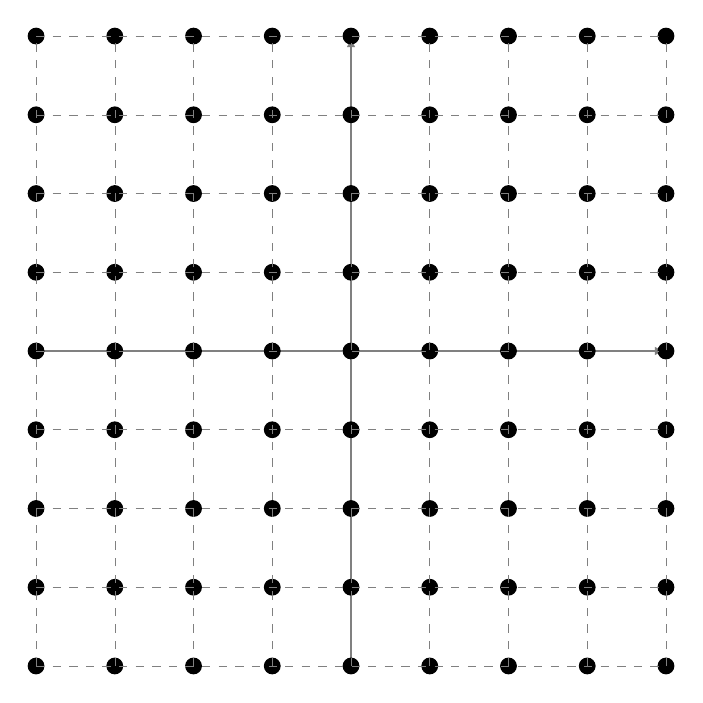
\begin{tikzpicture}[scale=1]
    \coordinate (Origin)   at (0,0);
    \coordinate (XAxisMin) at (-4,0);
    \coordinate (XAxisMax) at (4,0);
    \coordinate (YAxisMin) at (0,-4);
    \coordinate (YAxisMax) at (0, 4);
    \draw [thin, gray,-latex] (XAxisMin) -- (XAxisMax);% Draw x axis
    \draw [thin, gray,-latex] (YAxisMin) -- (YAxisMax);% Draw y axis

    %\clip (-3,-2) rectangle (10cm,10cm); % Clips the picture...
    \pgftransformcm{1}{0}{0}{1}{\pgfpoint{0cm}{0cm}}
          % This is actually the transformation matrix entries that
          % gives the slanted unit vectors. You might check it on
           % MATLAB etc. . I got it by guessing.
          % Draws a grid in the new coordinates.
    \foreach \x in {-4,-3,...,4}{% Two indices running over each
      \foreach \y in {-4,-3,...,4}{% node on the grid we have drawn 
        \node[draw,circle,inner sep=2pt,fill] at (\x,\y) {};
            % Places a dot at those points
      }
    }
    \draw[style=help lines,dashed] (-4,-4) grid[] (4,4);
  \end{tikzpicture}
  \caption{Vector Space $\R^2$ for $\forall (x,y); -4 \leq x \leq 4 and -4 \leq y \leq 4$.}
  \label{figure:solving-CVP-bad-basis}
\end{figure}


\section{Acknowledgements}
Almost none of this work is of my own. This work is from \textit{Linear Algebra} by George Shilov. And lecture notes from Dr. Matt Miller's MATH544H class taught at the University of South Carolina in the Spring of 2019.
\chapter{Week 1 Lectures}
\section{14 January 2019}
\begin{defn}
Linear Algebra is the study of vector spaces and the maps between them.
\end{defn}

\begin{defn}
A function $T:V\to W$, from vector space $V$, the domain, to vector space $W$, the codomain, is called a linear transformation if
\[T(c\Vec{u}+\Vec{v})=cT(\Vec{u})+T(\Vec{v});\ \forall \Vec{u},\Vec{v}\in V \wedge c\in \R\]
\end{defn}

\begin{ex}
\[T:\R\to\R;\ T(x)=2x\]
\[T(cu+v) = 2cu + v = cT(u)+T(v)\]
So this is a linear transformation.
\end{ex}
\begin{ex}
\[C^0[0,2\pi] = \{f:[0,2\pi]\to\R\ |\ f\ is \ continuous\}\]
\[S:C^0[0,2\pi]\to \R\]
\[S(f) = f(\pi)\]
Check linearity.
\[S(cf+g) = (cf+g)(\pi)=cf(\pi)+g(\pi)=cS(f)+S(g)\]
\end{ex}

\begin{ex}
\[Let\ T:C^0[0,2\pi]\to \R\]
\[T(f)=\Bar{f}\]
\[T(f)=\frac{1}{2\pi}\int_0^{2\pi}f(x)\ dx\]
Check linearity.
\[T(cf+g)=\frac{1}{2\pi}\int_0^{2\pi}(cf+g)(x)\ dx\]
\[T(cf+g)=\frac{1}{2\pi}(c\int_0^{2\pi}f(x)\ dx+\int_0^{2\pi}g(x)\ dx)\]
\[T(cf+g)=cT(f)+T(g)\]
\end{ex}

$\R^2$ and $\R^3$ are vector spaces, $(x,y)$ is mapped to the vector $\begin{bmatrix}x\\y
\end{bmatrix}$ and $(x,y,z)$ is mapped to the vector $\begin{bmatrix}x\\y\\z
\end{bmatrix}$.
\begin{ex}
Let $T:\R^2\to\R^3$ be defined by \[T(\begin{bmatrix}x\\y\end{bmatrix})=\begin{bmatrix}x+3y\\-x+y\\2x+y\end{bmatrix}\]
Verify linearity.
\[T(c\begin{bmatrix}x\\y\end{bmatrix}+\begin{bmatrix}z\\w\end{bmatrix})=T(\begin{bmatrix}cx+z\\cy+w\end{bmatrix}=\begin{bmatrix}cx+z+3cu+3w\\-cx-z+cy+w\\2cx+2z+cy+w\end{bmatrix}\]
\[T(c\begin{bmatrix}x\\y\end{bmatrix}+\begin{bmatrix}z\\w\end{bmatrix})=\begin{bmatrix}cx+3cu\\-cx+cy\\2cx+cy\end{bmatrix}+\begin{bmatrix}z+3w\\-z+w\\2z+w\end{bmatrix}\]
\[T(c\begin{bmatrix}x\\y\end{bmatrix}+\begin{bmatrix}z\\w\end{bmatrix})=c\begin{bmatrix}x+3u\\-x+y\\2x+y\end{bmatrix}+\begin{bmatrix}z+3w\\-z+w\\2z+w\end{bmatrix}\]
\[T(c\begin{bmatrix}x\\y\end{bmatrix}+\begin{bmatrix}z\\w\end{bmatrix})=cT(\begin{bmatrix}x\\y\end{bmatrix})+T(\begin{bmatrix}z\\w\end{bmatrix})\]
This transformation is the same as the matrix transformation, $\begin{bmatrix}1 & 3\\ -1 & 1\\ -2 & 1\end{bmatrix}$.
\end{ex}

\begin{defn}
Let $T: V\to W$ be a linear transformation. The range or image of $T$ is the is the set range $\mathscr{R}(T)$.
\begin{center}
    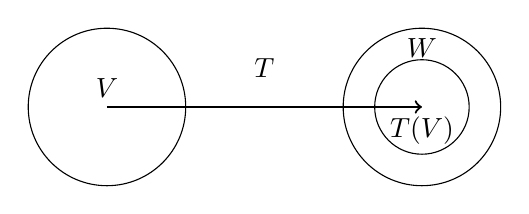
\begin{tikzpicture}
    \draw (1,0) ellipse (1cm and 1cm) node[above] {$V$};
    \draw (5,0) ellipse (1cm and 1cm);
    \draw (5,0.75) node {$W$};
    \draw (3,0.5) node {$T$};
    \draw[thick,->] (1,0) -- (5,0);
    \draw (5,0) ellipse (0.6 cm and 0.6cm) node[below] {$T(V)$};
    \end{tikzpicture}
\end{center}

\end{defn}
\section{16 January 2019}
\begin{defn}
Let $T: V\to W$ be a linear transformation. The range or image of $T$ is the is the set range $\mathscr{R}(T)=T(V)$=im(T).
\[\{\Vec{w}\in W\ |\ (\exists \Vec{v}\in V) \Vec{w}=T(\Vec{v})\}\]
\end{defn}
\begin{defn}
The kernel or nullspace of $T$ is $ker(T)=\mathscr{N}(T)$.
\[\{\Vec{v}\in V\ |\ T(V)=\Vec{0}_W\}\]
Note: The kernel is a vector space.
\end{defn}
\begin{center}
    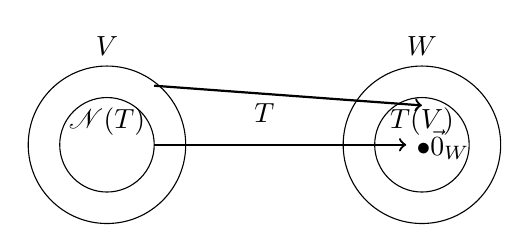
\begin{tikzpicture}
    \draw (1,0) ellipse (1cm and 1cm) node[above] {$\mathscr{N}(T)$};
    \draw (5,0) ellipse (1cm and 1cm);
    \draw (5,0) ellipse (0.6cm and 0.6cm) node[above] {$T(V)$};
    \draw (1,0) ellipse (0.6cm and 0.6cm);
    \draw (5,1.25) node {$W$};
    \draw (3,0.4) node {$T$};
    \draw (1,1.25) node {$V$};
    \draw[thick,->] (1.6,0) -- (4.8,0) node[right] {$\bullet\Vec{0}_W$};
    \draw[thick,->] (1.6,0.75)--(5.0,0.5);
    \end{tikzpicture}
\end{center}
\begin{bmatrix}
\end{bmatrix}
\begin{ex}
Let $T:\R^2\to\R^3;\ T(\begin{bmatrix}x\\y\end{bmatrix}) =
T(\begin{bmatrix}x+3y\\-x+y\\2x+y\end{bmatrix})$.
\[ker(T)=\{\begin{bmatrix}x\\y\end{bmatrix}\in \R^2\ |\ T(\begin{bmatrix}
x\\y\end{bmatrix})=\begin{bmatrix}
0\\0\\0
\end{bmatrix}\in \R^3\}\]
\[x+3y=0\]
\[-x+y=0\]
\[4y=0\implies y=0 \implies x=0\implies ker(T)=\{\begin{bmatrix}
0\\0
\end{bmatrix}\}\]
\[T(V)=\{\begin{bmatrix}
x+3y\\-x+y\\2x+y
\end{bmatrix}\ |\ x,y \in \R\}\]
\[T(V)=\{x\begin{bmatrix}
1\\-1\\2
\end{bmatrix}+y\begin{bmatrix}
3\\1\\1
\end{bmatrix}\ |\ x,y\in \R\}=\{t\Vec{a}+s\Vec{b}\ |\ t,s\in\R\}\]
Which plane is it? Contrast $L(\begin{bmatrix}
x\\y
\end{bmatrix})=\begin{bmatrix}
x\\y\\0
\end{bmatrix}$.\\
%\begin{center}
  \begin{tikzpicture}[scale=0.25]
    \coordinate (Origin)   at (0,0);
    \coordinate (XAxisMin) at (-4,0);
    \coordinate (XAxisMax) at (4,0);
    \coordinate (YAxisMin) at (0,-4);
    \coordinate (YAxisMax) at (0, 4);
    \draw [thin, gray,-latex] (XAxisMin) -- (XAxisMax);% Draw x axis
    \draw [thin, gray,-latex] (YAxisMin) -- (YAxisMax);% Draw y axis
    
    \draw [thin, gray,-latex] (5.5,0) -- (7.5,0);% Draw T
    
    \coordinate (Origin2)   at (12,0);
    \coordinate (XAxisMin2) at (8,0);
    \coordinate (XAxisMax2) at (16,0);
    \coordinate (YAxisMin2) at (12,-4);
    \coordinate (YAxisMax2) at (12, 4);
    \coordinate (ZAxisMax) at (13.5,2);
    \coordinate (ZAxisMin) at (10.5,-2);
    \draw [thin, gray,-latex] (XAxisMin2) -- (XAxisMax2);% Draw x axis
    \draw [thin, gray,-latex] (YAxisMin2) -- (YAxisMax2);% Draw y axis
    \draw [thin, gray,-latex] (ZAxisMin) -- (ZAxisMax);% Draw y axis

  \end{tikzpicture}
\end{center}
This is the plane, $3x-5y-4z=0$. This proves $T(V)\subseteq P$. To prove $T(V)=P$, we also need to prove $P\subseteq T(V)$.
\end{ex}
\section{16 January 2019 Dr. Miller Notes}
\begin{ex}
Let $T(\begin{bmatrix}
x\\y
\end{bmatrix})=\begin{bmatrix}
x+3y\\
-x+y\\
2x+y
\end{bmatrix}$.
\[im(T)=\{t\begin{bmatrix}
1\\-1\\2
\end{bmatrix}+s\begin{bmatrix}
3\\
1\\
1
\end{bmatrix}\ |\ t,s\in \R\}\]
We know that this is contained in the plane $3x-5y-4z$.\\
To see that $P\subseteq im(T)$, we solve
\[t+3s=x;\ -t+6=s;\ \]
\end{ex}

\section{18 January 2019}
\subsection{Gaussian Elimination}
\begin{ex}
Let \[\left \{
\begin{tabular}{cccc}
E_1: & x+y-z & =&1\\
E_2: & 2x-y+7z & =&8 \\
E_3: & -x+y-5z & = &-5
\end{tabular}\]
Solve for $(x,y,z)$. Find the intersection of 3 planes in $\R^3$. We happen to know that $(3,-2,0)$, and $(1,1,1)$ lie in the intersection.\\
Compute elimination: Let's make $E_2 : -2E_1+E_2$ and $E_3=E_1+E_3$.
\[\left \{
\begin{tabular}{cccc}
E_1: & x+y-z & =&1\\
E_2: & -3y+9z & =&6 \\
E_3: & 2y-6z & = &-4
\end{tabular}\]
Let's make $E_2 : \frac{-1}{3}E_2$ and $E_3=\frac{1}{2}E_3$.
\[\left \{
\begin{tabular}{cccc}
E_1: & x+y-z & =&1\\
E_2: & y-3z & =&-2 \\
E_3: & y-3z & = &-2
\end{tabular}\]
Let $E_3 : -E_2+E_3$, this allows us to free $z$.
\[\left \{
\begin{tabular}{cccc}
E_1: & x+y-z & =&1\\
E_2: & y-3z & =&-2 \\
E_3: & 0& = & 0
\end{tabular}\]
Then to solve it is just set $z=t$, for some $t\in\R$. And $y=-2+3z=-2+3t$, and $x=1+z-y=1+t-(-2t+3t)=3-2t$. So we get the parametric line,
$\left \{
\begin{tabular}{ccc}
x&=&3-2t\\
y&=&-2+3t\\
z&=&t
\end{tabular}$
\end{ex}
\hline
\subsection{Same example using Gaussian Elimination}
\begin{ex}
\[
\begin{tabular}{cccc}
E_1: & x+y-z & =&1\\
E_2: & 2x-y+7z & =&8 \\
E_3: & -x+y-5z & = &-5
\end{tabular} \implies \begin{amatrix}{3}1 & 1 & -1 & 1\\ 2 & -1 & 7 & 8\\ -1 & 1 & 7 & -5\end{amatrix}\]
This matrix with the vertical bar is called an \textit{Augmented Matrix} for $E_1, E_2, E_3$. \[A = \begin{bmatrix}1 & 1 & -1\\ 2 & -1 & 7\\ -1 & 1 & 7\end{bmatrix}\ B=\begin{bmatrix}1\\8\\-5\end{bmatrix}\]
In this example $A$ is called the \textit{Coefficient Matrix} and $B$ is called the \textit{Right Hand Side Matrix}.
\end{ex}
\subsection{Gaussian Row Operations}
There are 3 kinds of row operations that do not affect the solutions.
\begin{enumerate}
    \item $R_i \leftrightarrow R_j$ swap row i with row j.
    \item Replace row j with $cR_i+R_j$, leaving $R_i$ unchanged $(i\neq j)$.
    \item Replace $R_i$ by $cR_i$, some $c\neq 0$.
\end{enumerate}
\setcounter{ex}{1}
\begin{ex} Continued.
\[\begin{amatrix}{3}1 & 1 & -1 & 1\\ 2 & -1 & 7 & 8\\ -1 & 1 & 7 & -5\end{amatrix}\xrightarrow[R_1+R_2]{R_1+R_3}\begin{amatrix}{3}1 & 1 & -1 & 1\\ 0 & -3 & 9 & 6\\ 0 & 2 & -6 & -4\end{amatrix}\]
\[\xrightarrow[2R_3+R_2]{}\begin{amatrix}{3}1 & 1 & -1 & 1\\ 0 & 1 & -3 & -2\\ 0 & 2 & -6 & -4\end{amatrix}\xrightarrow[-2R_2 + R_3]{}\begin{amatrix}{3}1 & 1 & -1 & 1\\ 0 & 1 & -3 & -2\\ 0 & 0 & 0 & 0\end{amatrix}\]
\end{ex}
\hline
\subsection{Row Echelon Form}
\begin{enumerate}
    \item Rows with all 0's are on bottom.
    \item First non-zero entry, reading left to right right is a $1$.
    \item If $R_i, R_j$ are non-zero rows, $j>i$ then the leading $1$ in $R_j$ is to the right of the leading $1$ in $R_i$.
\end{enumerate}
\setcounter{ex}{1}
\begin{ex}Continued.
\[\begin{amatrix}{3}1 & 1 & -1 & 1\\ 0 & 1 & -3 & -2\\ 0 & 0 & 0 & 0\end{amatrix}\xrightarrow[R_2+R_1]{}\begin{amatrix}{3}1 & 0 & 2 & 3\\ 0 & 1 & -3 & -2\\ 0 & 0 & 0 & 0\end{amatrix}\]
\end{ex}
\hline
\subsection{Reduced Row Echelon Form}
Only 0's above the leading 1's.
\setcounter{ex}{1}
\begin{ex}Continued\\
Now undo the matrix, to get solution equations.
\[\left \{ \begin{tabular}{c}
x+2z=3\\
y-3z=-2
\end{tabular}\]
\end{ex}

\begin{ex}
\[\begin{amatrix}{3}
1 & 0 & 0 & 4\\
0 & 1 & 0 & -1\\
0 & 0 & 1 & 0\\
0 & 0 & 0 & 0
\end{amatrix} \implies \begin{tabular}{c}
     x=4\\y=-1\\z=0\\0=0
\end{tabular}\] So this means that the solution is a line from $(4,-1,0,t)$ for all $t\in \R$.
\end{ex}
\begin{ex}
\[\begin{amatrix}{4}
1 & 2 & 0 & 3 & 3\\
0 & 0 & 1 & -1 & 0\\
0 & 0 & 0 & 0 & 0
\end{amatrix} \implies \begin{tabular}{c}
     x+2y+3w=3\\z-w=0\\z0=0
\end{tabular}\] So this means that x and z are bound because they are the leading 1's, and other variables are free, and can be assigned to anything in the universal set.
\end{ex}

\begin{ex}
\[\begin{amatrix}{3}
1 & 0 & 2 & 3\\
0 & 1 & 1 & -4\\
0 & 0 & 0 & 1
\end{amatrix} \implies \begin{tabular}{c}
     x+2z=3\\y+z=-4\\0=1
\end{tabular}\] So this means we have 0 solutions, because $0=1$ is a contradiction.
\end{ex}
\subsection{Note} The variables in columns with leading 1's are the bound variables. The other variables are free variables, and can be set to anything.
\chapter{Week 2 Lectures}
\chapter{Definitions}
\begin{defn}
A field is a set $\F$ with operations of addition $(+)$ and multiplication $(\cdot)$ and distinct elements: $0$, $1$ so that
\begin{enumerate}
    \item[(C1)] Closure under addition: if $a,b\in\F$ then $a+b\in\F$.
    \item[(C2)] Closure under multiplication: if $a,b\in\F$ then $a\cdot b\in \F$.
    \item[(A1)] Addition is commutative, $a+b=b+a$ for all $a,b\in\F$.
    \item[(A2)] Addition is associative, $(a+b)+c=a+(b+c)$, for all $a,b,c\in\F$.
    \item[(A3)] There exists a $0$ identity, $a+0=0+a=a$, for all $a\in\F$.
    \item[(A4)] For each $a\in\F$ there exists an element $b$ so that $a+b=b+a=0$.\\
    This element is indeed unique, and we write it as $b=-a$.
    \item[(M1)] Multiplication is commutative, $ab=ba$ for all $a,b\in\F$.
    \item[(M2)] Multiplication is associative, $a(bc)=(ab)c$ for all $a,b,c\in\F$.
    \item[(M3)] There exists a $1$ identity, $1a=a$, for all $a\in\F$.
    \item[(M4)] For each $a\in\F\setminus \{0\}$ there exists an element so that $ab=ba=1$.\\
    This element is indeed unique, and we write it as $b=a^{-1}$.
    \item[(D)] For all $a,b,c\in\F$, multiplication is distributive, $a(b+c)=ab+ac$.
 \end{enumerate}
\end{defn}
\begin{defn}
A set $V$ with binary operations $(+)$ and scalar multiplication is called a vector space over a field $\F$ if:
\begin{enumerate}
    \item[(C1)] The set is closed under addition, for all $\vu,\vv\in V$, $\vu + \vv \in V$.
    \item[(C2)] The set is closed under scalar multiplication, for all $c\in\F$ and $\vu\in V$, $c\vu \in V$.
    \item[(A1)] Vector addition is commutative, $\vu+\vv = \vv + \vu$, for all $\vu,\vv \in V$.
    \item[(A2)] Vector addition is commutative, $(\vu+\vv)+\vw=\vu+(\vv+\vw)$, for all $\vu,\vv,\vw\in V$.
    \item[(A3)] There is an element $\Vec{0}\in V$, so that $\vec{0}+\vu=\vu+\vec{0}$ for all $\vu\in V$.
    \item[(A4)] For every $\vu\in V$ there exists a vector $\vv\in V$ so that $\vu+\vv=\vec{0}$.\\
    We write $\vv=-\vu$.
    \item[(S1)] Scalar multiplication is associative, $s\cdot(t\cdot\vu)=(s\cdot t)\cdot\vu$ for all $s,t\in \F$ and $\vu\in V$.
    \item[(S2)] Recall that we have $1\in\F$, then $1\cdot \vu=\vu$ for all $\vu\in V$.
    \item[(D1)] $c(\vu+\vv)=c\vu+c\vv$ for all $c\in \F$, $\vu,\vv\in V$.
    \item[(D2)] $(c+d)\vu=c\vu+d\vu$ for all $c\in\F$, $\vu\in V$.
\end{enumerate}
\end{defn}

\section{14 January 2019}
\begin{defn}
Linear Algebra is the study of vector spaces and the maps between them.
\end{defn}

\begin{defn}
A function $T:V\to W$, from vector space $V$, the domain, to vector space $W$, the codomain, is called a linear transformation if
\[T(c\Vec{u}+\Vec{v})=cT(\Vec{u})+T(\Vec{v});\ \forall \Vec{u},\Vec{v}\in V \wedge c\in \R\]
\end{defn}

\begin{ex}
\[T:\R\to\R;\ T(x)=2x\]
\[T(cu+v) = 2cu + v = cT(u)+T(v)\]
So this is a linear transformation.
\end{ex}
\begin{ex}
\[C^0[0,2\pi] = \{f:[0,2\pi]\to\R\ |\ f\ is \ continuous\}\]
\[S:C^0[0,2\pi]\to \R\]
\[S(f) = f(\pi)\]
Check linearity.
\[S(cf+g) = (cf+g)(\pi)=cf(\pi)+g(\pi)=cS(f)+S(g)\]
\end{ex}

\begin{ex}
\[Let\ T:C^0[0,2\pi]\to \R\]
\[T(f)=\Bar{f}\]
\[T(f)=\frac{1}{2\pi}\int_0^{2\pi}f(x)\ dx\]
Check linearity.
\[T(cf+g)=\frac{1}{2\pi}\int_0^{2\pi}(cf+g)(x)\ dx\]
\[T(cf+g)=\frac{1}{2\pi}(c\int_0^{2\pi}f(x)\ dx+\int_0^{2\pi}g(x)\ dx)\]
\[T(cf+g)=cT(f)+T(g)\]
\end{ex}

$\R^2$ and $\R^3$ are vector spaces, $(x,y)$ is mapped to the vector $\begin{bmatrix}x\\y
\end{bmatrix}$ and $(x,y,z)$ is mapped to the vector $\begin{bmatrix}x\\y\\z
\end{bmatrix}$.
\begin{ex}
Let $T:\R^2\to\R^3$ be defined by \[T(\begin{bmatrix}x\\y\end{bmatrix})=\begin{bmatrix}x+3y\\-x+y\\2x+y\end{bmatrix}\]
Verify linearity.
\[T(c\begin{bmatrix}x\\y\end{bmatrix}+\begin{bmatrix}z\\w\end{bmatrix})=T(\begin{bmatrix}cx+z\\cy+w\end{bmatrix}=\begin{bmatrix}cx+z+3cu+3w\\-cx-z+cy+w\\2cx+2z+cy+w\end{bmatrix}\]
\[T(c\begin{bmatrix}x\\y\end{bmatrix}+\begin{bmatrix}z\\w\end{bmatrix})=\begin{bmatrix}cx+3cu\\-cx+cy\\2cx+cy\end{bmatrix}+\begin{bmatrix}z+3w\\-z+w\\2z+w\end{bmatrix}\]
\[T(c\begin{bmatrix}x\\y\end{bmatrix}+\begin{bmatrix}z\\w\end{bmatrix})=c\begin{bmatrix}x+3u\\-x+y\\2x+y\end{bmatrix}+\begin{bmatrix}z+3w\\-z+w\\2z+w\end{bmatrix}\]
\[T(c\begin{bmatrix}x\\y\end{bmatrix}+\begin{bmatrix}z\\w\end{bmatrix})=cT(\begin{bmatrix}x\\y\end{bmatrix})+T(\begin{bmatrix}z\\w\end{bmatrix})\]
This transformation is the same as the matrix transformation, $\begin{bmatrix}1 & 3\\ -1 & 1\\ -2 & 1\end{bmatrix}$.
\end{ex}

\begin{defn}
Let $T: V\to W$ be a linear transformation. The range or image of $T$ is the is the set range $\mathscr{R}(T)$.
\begin{center}
    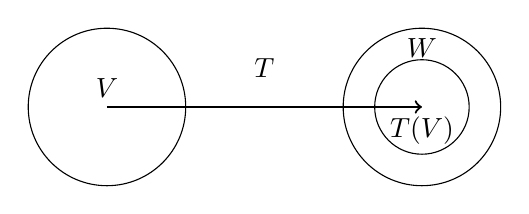
\begin{tikzpicture}
    \draw (1,0) ellipse (1cm and 1cm) node[above] {$V$};
    \draw (5,0) ellipse (1cm and 1cm);
    \draw (5,0.75) node {$W$};
    \draw (3,0.5) node {$T$};
    \draw[thick,->] (1,0) -- (5,0);
    \draw (5,0) ellipse (0.6 cm and 0.6cm) node[below] {$T(V)$};
    \end{tikzpicture}
\end{center}

\end{defn}
\end{document}